\section{体感速度モデルの提案}
これまで、スケールスピードと実速度を比較することで、体感速度はスケールスピードと一致せず、単なるスケール比に一致することが明らかになった。
さらに、その過程において体感速度を変化させるパラメータを発見した。列挙した中で最も影響力のあるパラメータが、走行映像のクロップ率やカメラの画角・ドライバの視野角であることが明らかになった。
そこで、走行映像のクロップ率とドライバの視野角を体感速度変化のパラメータとして、体感速度を定式化する手法を提案する。本研究では、実測値との比較として、視野角・ディスプレイ比等、DS環境におけるパラメータを定数とした
幾何学計算による幾何学モデルを提案する。

\subsection{原理}
実車が同じ速度で走行する場合でも、視野角が広い方が、体感速度が速く感じるという現象が生じる基準視野角と、ある視野角での画面上の一方から他方の点にかけてのピクセルの移動距離の比が体感速度の比となる。
図\ref{taikan:pixel}に、ピクセルの移動距離の考え方を示す。
同様の原理として、交通事故で取り上げられるコリジョンコース現象が挙げられる。複数の走行映像において、ピクセルの移動速度が一致する時、体感速度の比と一致していることが望ましい。

\begin{figure}[h]
  \begin{center}
  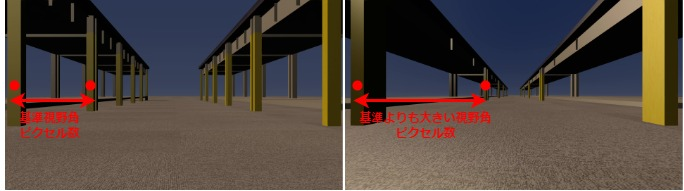
\includegraphics[width=.65\linewidth]{img/11.jpg}
  \caption{ピクセルの移動距離の考え方}
  \label{taikan:pixel}
  \end{center}
\end{figure}

\clearpage
\subsection{体感速度モデルの定式化}
体感速度を求めるために、映像中のポール間の移動の際に映像中の移動ピクセル数と、環境によって決まるパラメータを定式化する。
ここでは、体感速度$v_{sense}$を、視野角の関数$f(h_{fov_v})$で表し、$h_{fov_v}$を、クロップ率の関数$g(n)$で表すことを目標とする。
実際の速度\verb|(実速度とする)|を$v_2$とすると、式\eqref{taikan:eq:model1}、\eqref{taikan:eq:model2}に示す関係式を求める。

\begin{align}
  v_{sense} = f(h_{fov_v})\cdot v_s = f(g(n))\cdot v_s \label{taikan:eq:model1}\\
  h_{fov_v} = g(n) \label{taikan:eq:model2}
\end{align}

まず、ディスプレイのアスペクト比とサイズ(ディスプレイの対角線の長さ)をディスプレイの縦・横の長さに変換する式を式\eqref{taikan:eq:dis1}、\eqref{taikan:eq:dis2}に示す。図\ref{taikan:displaytosize}
にディスプレイ長さの概要と諸条件を示す。

\begin{figure}[h]
  \begin{center}
  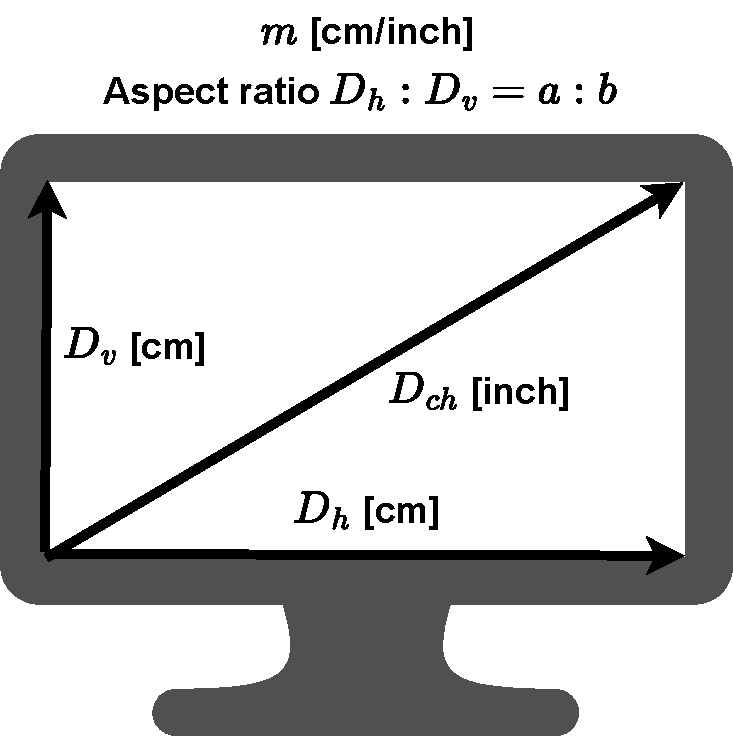
\includegraphics[width=.65\linewidth]{img/12.pdf}
  \caption{ディスプレイ長さの概要と諸条件}
  \label{taikan:displaytosize}
  \end{center}
\end{figure}

\begin{align}
    D_v = D_{ch} \cdot m \cdot \frac{b}{\sqrt{a^2+b^2}} \label{taikan:eq:dis1}\\
    D_h = D_{ch} \cdot m \cdot \frac{a}{\sqrt{a^2+b^2}} \label{taikan:eq:dis2}
\end{align}

$D_v$:ディスプレイの縦の長さ\si{[cm]}、$D_h$:ディスプレイの横の長さ\si{[cm]}、$D_{ch}$:ディスプレイの対角線の長さ\si{[inch]}、
$m$:2.4\si{[cm/inch]}、$a$:ディスプレイの横のアスペクト比:16、$b$:ディスプレイの縦のアスペクト比:9

次に、ディスプレイの縦・横の長さとディスプレイとの視点距離をDS上での水平・垂直方向の基準視野角に式\eqref{taikan:eq:kijun1}、\eqref{taikan:eq:kijun2}を用いて変換する。
図\ref{taikan:kijuntods}に基準視野角とその導出の諸条件を示す。


\begin{figure}[h]
  \begin{center}
  \subfigure[水平方向]{
  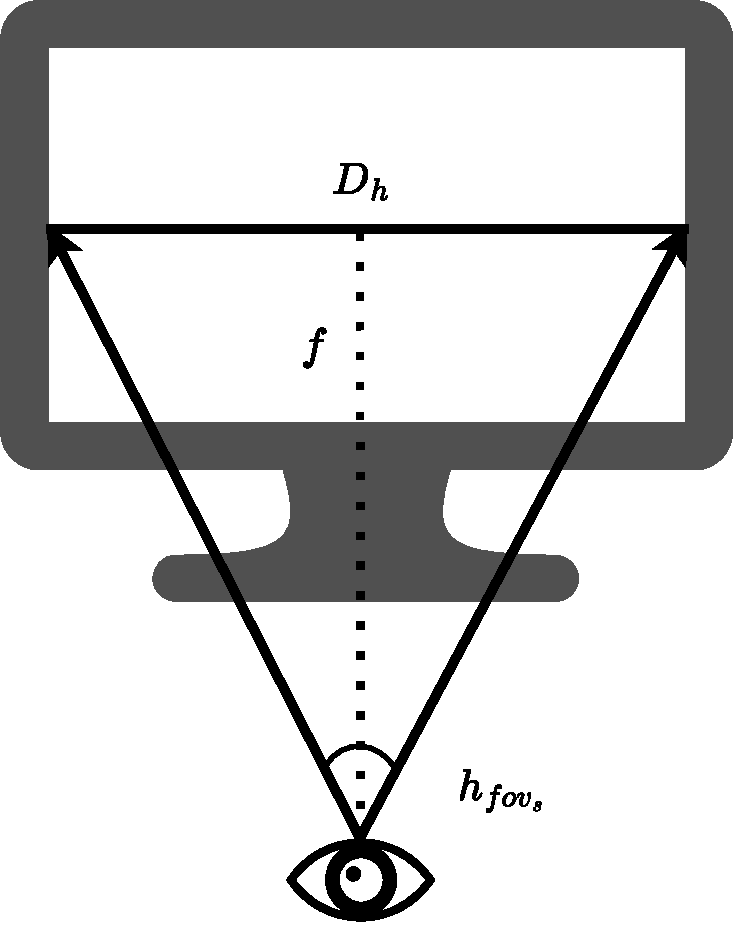
\includegraphics[width=.4\columnwidth]{img/13_1.pdf}
  \label{taikan:kijuntods1}
  }
  \subfigure[垂直方向]{
  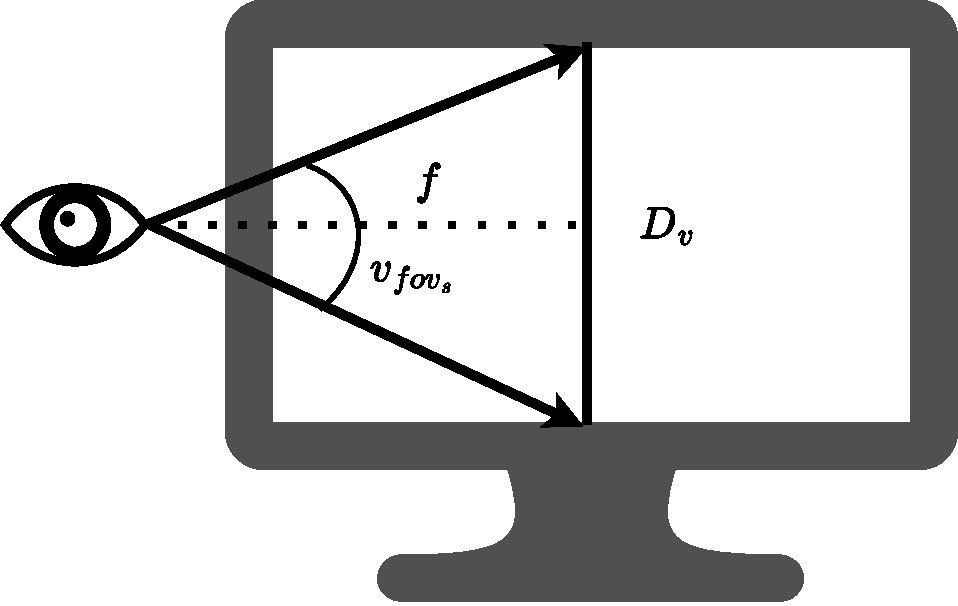
\includegraphics[width=.52\columnwidth]{img/13_2.pdf}
  \label{taikan:kijuntods2}
  }
  \caption{基準視野角とその導出の諸条件}
  \label{taikan:kijuntods}
\end{center}
\end{figure}

\begin{align}
    h_{fov_s} = 2\tan{\frac{D_h}{2f}} \label{taikan:eq:kijun1}\\
    v_{fov_s} = 2\tan{\frac{D_v}{2f}} \label{taikan:eq:kijun2}
\end{align}

$h_{fov_s}$:基準水平視野角\si{[degree]}、$v_{fov_s}$:基準垂直視野角\si{[degree]}、$f$:視点距離\si{[cm]}

次に、基準視野角を映像クロップによる視野角に変換する。クロップ率$n$の値域は、$1 \leqq n \leqq 3.5$とする。
$n = 1$の時$h_{fov_s}$、$v_{fov_s}$(基準視野角)とする。
式\eqref{taikan:eq:crop1}、\eqref{taikan:eq:crop2}は、映像のクロップにより、視野範囲が変わることを意味する。
クロップは縦横比を一定とし、映像の中心は変化させない。図\ref{taikan:shiyatocrop}に映像クロップによる視野角とその導出の諸条件を示す。
\clearpage
\begin{figure}[h]
  \begin{center}
  \subfigure[水平方向]{
  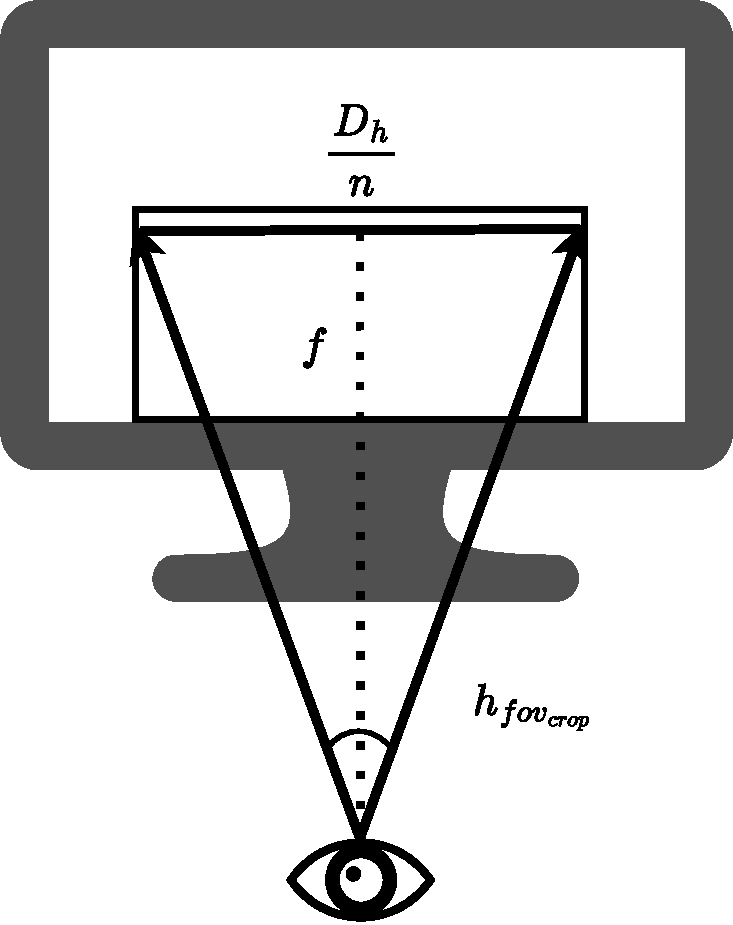
\includegraphics[width=.4\columnwidth]{img/14_1.pdf}
  \label{taikan:shiyatocrop1}
  }
  \subfigure[垂直方向]{
  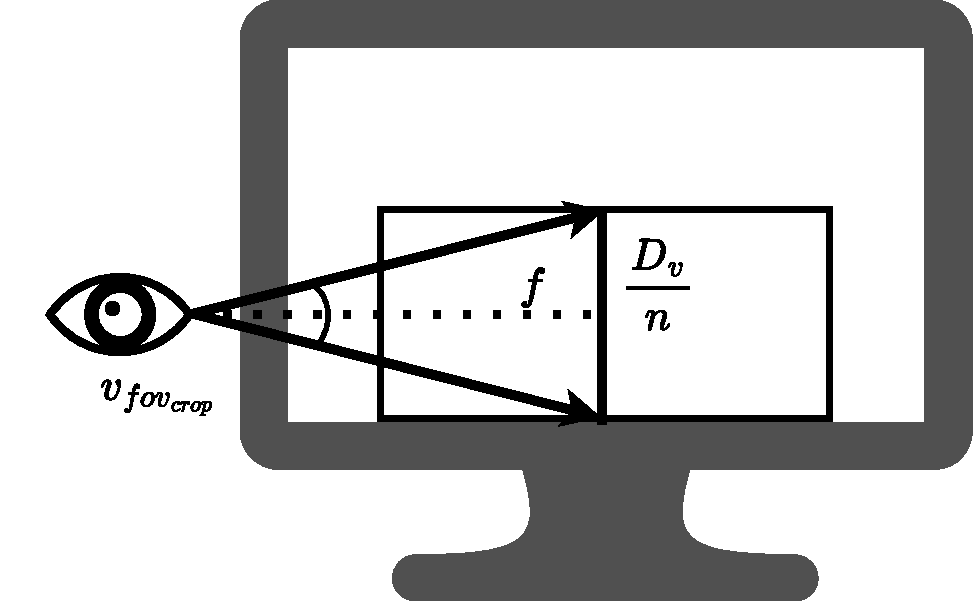
\includegraphics[width=.52\columnwidth]{img/14_2.pdf}
  \label{taikan:shiyatocrop2}
  }
  \caption{映像クロップによる視野角とその導出の諸条件}
  \label{taikan:shiyatocrop}
  \end{center}
\end{figure}

\begin{align}
  h_{fov_{crop}} = 2\tan{\frac{D_h}{2f\cdot n}} \label{taikan:eq:crop1}\\
  v_{fov_{crop}} = 2\tan{\frac{D_v}{2f\cdot n}} \label{taikan:eq:crop2}
\end{align}

$h_{fov_{crop}}$:映像クロップによる水平視野角\si{[degree]}、$v_{fov_{crop}}$:映像クロップによる垂直視野角\si{[degree]}、$n$:クロップ率の関数

次に、変数の視野角を基準よりも大きくとる場合に拡張する。つまり、$n<1$を考える。$n = 0.2 \thicksim 1$として拡張し、得られた視野角を変数
$h_{fov_v}$、$v_{fov_v}$とおく、これを体感速度のパラメータとする。$n$は、クロップ率を基準視野角から拡大または縮小するための値として拡張した、視野角拡大率とする。
$n$は、$h_{fov_v}$、$v_{fov_v}$のパラメータである。つまり、体感速度$v_{sense} = f(h_{fov_v}) = f(g(n))$とし、$h_{fov_v}=g(n)$である。
これらの式を、式\eqref{taikan:eq:kakudai1}、\eqref{taikan:eq:kakudai2}に示す。

\begin{align}
  h_{fov_v} = 2\tan{\frac{D_h}{2f\cdot n}} \label{taikan:eq:kakudai1}\\
  v_{fov_v} = 2\tan{\frac{D_v}{2f\cdot n}} \label{taikan:eq:kakudai2}
\end{align}

$h_{fov_v}$:水平視野角変数\si{[degree]}、$v_{fov_v}$:垂直視野角変数\si{[degree]}、$n$:視野角拡大率

次に、体感速度は、基準視野角と水平視野角変数におけるそれぞれの映像のポール間ピクセル数の比を、実速度に乗ずることで式\eqref{taikan:eq:vsense}により求められる。

\begin{align}
  v_{sense} = \frac{px_v}{px_s}v_s = m_{sense}\cdot v_s \label{taikan:eq:vsense}
\end{align}

$px_v$:$h_{fov_v}$におけるポール間ピクセル数\si{[px]} (実測値)、$px_s$:$h_{fov_s}$におけるポール間ピクセル数\si{[px]}実測値、$v_{sense}$:体感速度\si{[km/h]}、$v_s$:実速度\si{[km/h]}、$m_{sense}$:ポール間ピクセル数の比

図\ref{taikan:px}に視野角の違いによるポール間ピクセル数の違いを示す。

\begin{figure}[h]
  \begin{center}
  \subfigure[基準視野角]{
  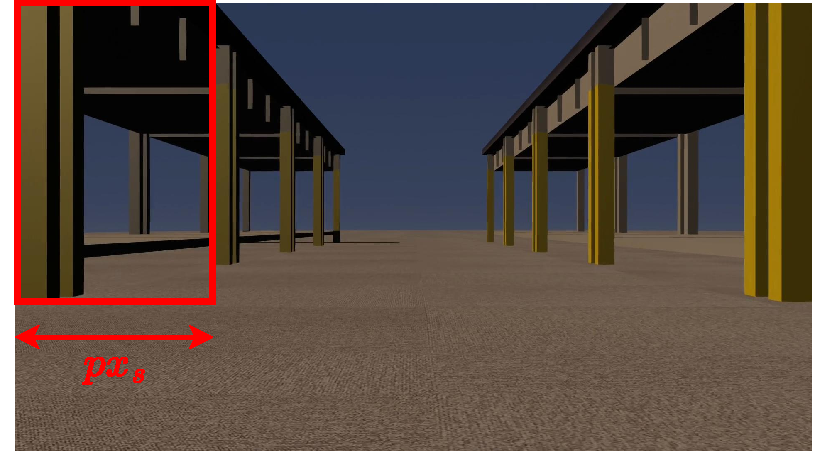
\includegraphics[width=.8\columnwidth]{img/15_1.pdf}
  \label{taikan:pxs}
  }
  \subfigure[変化視野角(増加)]{
  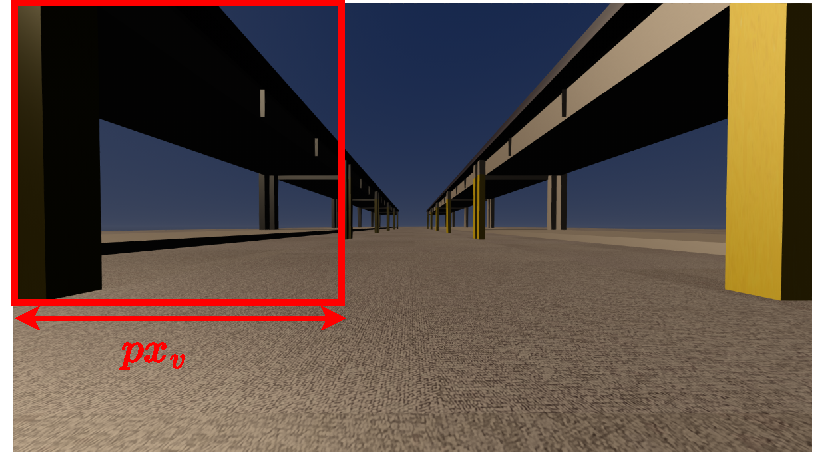
\includegraphics[width=.8\columnwidth]{img/15_2.pdf}
  \label{taikan:pxv}
  }
  \caption{視野角の違いによるポール間ピクセル数の違い}
  \label{taikan:px}
  \end{center}
\end{figure}

次に、$v_{sense}=f(h_{fov_v})$となる$f$を導きたい。$v_s$は一定として考えているため、$m_{sense}=f(h_{fov_v})$を導く。ここで、
視野角変数$h_{fov_v}$において、映像中のボールが画面の端にあるとする。(視点とディスプレイの短辺は$h_{fov_v}$の角度をなす。)
そこから、次のボールが画面の端になるように縦横比一定でクロップした時のクロップ率を視野辺ピクセル倍率$n_{p_{\to}p}$とする。
基準視野角においても同様に、$n_{p_{\to}p_s}$(基準視野角の場合の$n_{p_{\to}p_s}$)を求める。なお、遠近法より、$n_{p_{\to}p_s} = 2$であることが一般的に知られている。すると、
$m_{sense}$は、図\ref{taikan:kika}に示す視野角に関する幾何学を用いて、式\eqref{taikan:eq:kika1}\verb|~|\eqref{taikan:eq:kika3}のように求めることができる。

\begin{align}
  px_s = \frac{h_{px}}{2} - \frac{h_{px}}{2}\Bigg(\frac{\tan\frac{h_{fov_s}}{2\cdot n_{p_{\to}p_s}}}{\tan{\frac{h_{fov_s}}{2}}}\Bigg) = \frac{h_{px}}{2}\Biggl(1-\frac{\tan{\frac{h_{fov_s}}{4}}}{\tan{\frac{h_{fov_s}}{2}}}\Biggr) \label{taikan:eq:kika1}\\
  px_v = \frac{h_{px}}{2} - \frac{h_{px}}{2}\Bigg(\frac{\tan\frac{h_{fov_v}}{2\cdot n_{p_{\to}p_v}}}{\tan{\frac{h_{fov_v}}{2}}}\Bigg) = \frac{h_{px}}{2}\Biggl(1-\frac{\tan{\frac{h_{fov_v}}{2\cdot n_{p_{\to}p}}}}{\tan{\frac{h_{fov_v}}{2}}}\Biggr) \label{taikan:eq:kika2}\\
  m_{sense} = \frac{px_v}{px_s} = \frac{\Biggl\{\frac{h_{px}}{2}\Bigg(1-\frac{\tan\frac{h_{fov_v}}{2\cdot n_{p_{\to}p}}}{\tan\frac{h_{fov_v}}{2}}\Bigg)\Biggr\}}{\Biggl\{\frac{h_{px}}{2}\Bigg(1-\frac{\tan\frac{h_{fov_s}}{4}}{\tan\frac{h_{fov_s}}{2}}\Bigg)\Biggr\}} = \frac{1-\frac{\tan\frac{h_{fov_v}}{2\cdot n_{p_{\to}p}}}{\tan\frac{h_{fov_s}}{2}}}{1-\frac{\tan\frac{h_{fov_s}}{4}}{\tan\frac{h_{fov_s}}{2}}} \label{taikan:eq:kika3}
\end{align}

